\documentclass[11pt]{article}
\usepackage[a4paper,margin=1in]{geometry}
\usepackage{amsmath,amssymb,amsthm}
\usepackage{graphicx}
\usepackage{hyperref}

\newtheorem{theorem}{Theorem}
\newtheorem{corollary}{Corollary}

\newcommand{\N}{\mathbb N}
\newcommand{\R}{\mathbb R}
\newcommand{\linf}{\ell_\infty}
\newcommand{\co}{c_0}
\newcommand{\X}{\ell_\infty/c_0}

\title{A CH obstruction to lifting automorphisms modulo locally null operators}
\author{Run \texttt{fa\_banach\_001}, agent lane 12}
\date{2026-06-20}

\begin{document}
\maketitle

\section*{Source and target problem}

The source paper is Piotr Koszmider and Cristobal Rodriguez-Porras,
\emph{On automorphisms of the Banach space \(\ell_\infty/c_0\)},
arXiv:1501.03466 \cite{KRP}.

In Problem 7.1, the authors ask whether it is consistent, possibly under PFA
or OCA+MA, that every automorphism \(T:\X\to\X\) can be represented as
\[
T=[R]+S,
\]
where \(R:\linf\to\linf\) induces an operator \([R]\) on the quotient and
\(S:\X\to\X\) is locally null.

\begin{center}

\includegraphics[width=0.95\linewidth]{figures/open_problem_crop.png}
\end{center}

\section*{Source ingredients}

The argument uses two results from the source paper.  First, Corollary 4.9
states that every liftable isomorphic embedding of \(\X\) into itself is
right-locally trivial.

\begin{center}
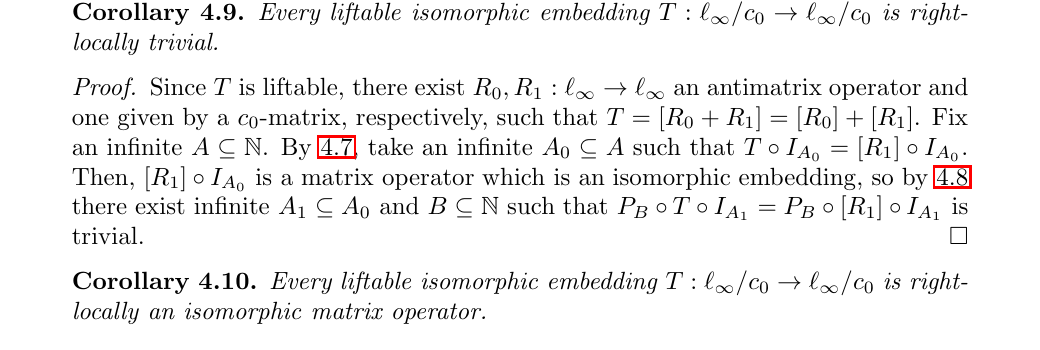
\includegraphics[width=0.95\linewidth]{figures/source_corollary_4_9_crop.png}
\end{center}

Second, Theorem 6.9 states that, under CH, there is a nowhere trivial
automorphism of \(\X\).

\begin{center}
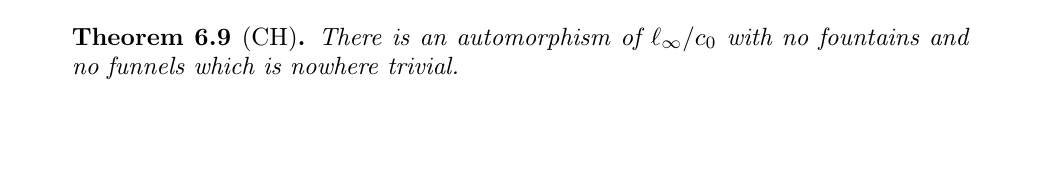
\includegraphics[width=0.95\linewidth]{figures/source_ch_theorem_6_9_crop.png}
\end{center}

\section*{Idea of the proof}

The key point is that locally null errors vanish after passing to an infinite
coordinate subspace.  If \(T=[R]+S\) and \(S\) is locally null, then on some
\(\ell_\infty(A)/c_0(A)\) we have \(S I_A=0\), hence \(T I_A=[R]I_A\).
Since \(T\) is an automorphism, this restriction of \([R]\) is a liftable
isomorphic embedding.  The source Corollary 4.9 then forces a further
restriction to be trivial.  Therefore \(T\) must be somewhere trivial.

\begin{theorem}
Let \(T:\X\to\X\) be an automorphism.  If
\[
T=[R]+S
\]
for some quotient-induced operator \([R]\) and some locally null operator
\(S:\X\to\X\), then \(T\) is somewhere trivial.
\end{theorem}

\begin{proof}
Let \(I_A:\ell_\infty(A)/c_0(A)\to\X\) and
\(P_B:\X\to\ell_\infty(B)/c_0(B)\) denote the standard coordinate inclusion
and projection.

Since \(S\) is locally null, applying the definition to \(A=\N\) gives an
infinite \(A_0\subseteq\N\) such that
\[
S I_{A_0}=0.
\]
Consequently
\[
T I_{A_0}=[R]I_{A_0}.
\]
Because \(T\) is an automorphism, \(T I_{A_0}\) is an isomorphic embedding of
\(\ell_\infty(A_0)/c_0(A_0)\) into \(\X\).  Therefore \([R]I_{A_0}\) is also
an isomorphic embedding, and it is liftable by restriction of the same lifting
\(R\) to the coordinates in \(A_0\).

Identify \(\ell_\infty(A_0)/c_0(A_0)\) with \(\X\) through any bijection
\(\N\to A_0\).  Corollary 4.9 of the source paper applies to this liftable
isomorphic embedding.  Hence there are infinite sets
\(A_1\subseteq A_0\), \(B\subseteq\N\), a bijection \(\sigma:B\to A_1\), and
a nonzero scalar \(r\in\R\) such that
\[
P_B [R] I_{A_1}([f])=[r f\circ\sigma]
\qquad (f\in\ell_\infty(A_1)).
\]
But \(S I_{A_1}=0\), so \(P_B T I_{A_1}=P_B[R]I_{A_1}\).  Thus \(T\) is
somewhere trivial.
\end{proof}

\begin{corollary}[CH]
Assuming the continuum hypothesis, there is an automorphism
\(T:\X\to\X\) which cannot be written as \(T=[R]+S\) with \(S\) locally null.
\end{corollary}

\begin{proof}
By Theorem 6.9 of the source paper, CH yields an automorphism \(T:\X\to\X\)
which is nowhere trivial.  The theorem above shows that any automorphism
admitting a decomposition \(T=[R]+S\) with \(S\) locally null must be somewhere
trivial.  Hence this CH automorphism admits no such decomposition.
\end{proof}

\section*{Scope and limitations}

This is a partial negative result.  It does not answer whether PFA or OCA+MA
implies the lifting-modulo-locally-null property.  Instead it proves the ZFC
implication
\[
\text{liftable modulo locally null} \quad\Longrightarrow\quad
\text{somewhere trivial}
\]
for automorphisms, and then combines this implication with the source paper's
CH nowhere-trivial automorphism.

Equivalently, a positive answer to Problem 7.1 under PFA or OCA+MA would imply
a positive answer to the later somewhere-triviality problem for automorphisms
under the same axiom.

\section*{Novelty check}

On 2026-06-20, I searched for exact phrases around
\[
\texttt{ell\_infty/c\_0 locally null automorphism lift modulo}
\]
and around \(\X\), ``somewhere trivial'', and ``locally null operator''.
The only direct hit found for the exact target was the source arXiv paper.

\section*{Human review recommendation}

Review this as a likely valid partial result.  The main point to check is that
the source Corollary 4.9 applies after replacing the domain by
\(\ell_\infty(A_0)/c_0(A_0)\), which is canonically isomorphic to \(\X\) after
choosing a bijection \(\N\to A_0\).

\begin{thebibliography}{9}
\bibitem{KRP}
Piotr Koszmider and Cristobal Rodriguez-Porras,
\emph{On automorphisms of the Banach space \(\ell_\infty/c_0\)},
arXiv:1501.03466, 2015.
\end{thebibliography}

\end{document}
